\documentclass[a4paper,12pt]{article}

\usepackage[utf8]{inputenc}
\usepackage[T1]{fontenc}
\usepackage{lmodern}
\usepackage{tikz}
\usetikzlibrary{positioning, arrows.meta, fit, shadows, backgrounds}
\usepackage{geometry}
\geometry{a4paper, margin=0.5in}
\usepackage{graphicx}
\usepackage{parskip}
\usepackage{enumitem}
\usepackage{hyperref}
\usepackage{times}
\usepackage{microtype}
\usepackage{eso-pic}
\usepackage[absolute,overlay]{textpos}

\begin{document}

\newpage
\mbox{}
\AddToShipoutPictureBG*{%
  \AtPageLowerLeft{
    \put(0,0){\includegraphics[width=\paperwidth,height=\paperheight]{background.jpg}}
  }%
}

\thispagestyle{empty}

\setlength{\TPHorizModule}{1mm}
\setlength{\TPVertModule}{1mm}

\begin{textblock*}{50mm}(112mm, 29mm)
  \textbf{December}
\end{textblock*}

\begin{textblock*}{50mm}(145mm, 29mm)
  \textbf{2025}
\end{textblock*}

\begin{textblock*}{100mm}(95mm, 45mm)
  \textbf{Mark L F Tlau}
\end{textblock*}

\begin{textblock*}{100mm}(95mm, 55mm)
  \textbf{2550670762}
\end{textblock*}

\begin{textblock*}{100mm}(95mm, 66mm)
  \textbf{BCA\_NEW}
\end{textblock*}

\begin{textblock*}{100mm}(95mm, 76mm)
  \textbf{BCS111}
\end{textblock*}

\begin{textblock*}{100mm}(95mm, 85mm)
  \textbf{07162P}
\end{textblock*}

\begin{textblock*}{100mm}(95mm, 95mm)
  \textbf{Mohyal Education and Research Institute, Qutab Institutional Area, New Delhi}
\end{textblock*}

\begin{textblock*}{100mm}(95mm, 109mm)
  \textbf{+916009341754}
\end{textblock*}

\begin{textblock*}{100mm}(95mm, 119mm)
  \textbf{wintersunset95@gmail.com}
\end{textblock*}

\begin{textblock*}{100mm}(122mm, 144mm)
  \textbf{(Yes)}
\end{textblock*}

\clearpage

\textbf{Q1:}
\begin{enumerate}
    \item \textbf{Trace the evolution of computers from mechanical calculators to the fifth generation, and identify how each
    technological shift enabled a new kind of real\-world application.} \\
    \llap{\textbf{Answer:}}
    The evolution of computers is a story of technological shifts, each enabling new real-world applications. The \textbf{Mechanical Era (1600s-1900s)}, based on gears and levers, first enabled the automation of calculation for mathematical tables. The \textbf{First Generation (1940s-1950s)} shifted to \textit{vacuum tubes}, allowing for massive, complex electronic calculations, which were applied to military ballistics (ENIAC) and scientific research. The move to smaller, more reliable \textit{transistors} marked the \textbf{Second Generation (1950s-1960s)}, reducing cost and enabling the first commercial business applications like payroll and inventory management. \textbf{Third Generation (1960s-1970s)} computers were built on the \textit{Integrated Circuit (IC)}, which led to minicomputers (like the DEC PDP-8) and brought computing to smaller businesses and university labs. The \textbf{Fourth Generation (1970s-Present)} began with the \textit{microprocessor}, putting an entire CPU on one chip. This shift democratized computing, enabling the personal computer (PC) and its applications like word processors, spreadsheets, and the internet. Finally, the \textbf{Fifth Generation (Present \& Future)} is defined by \textit{Parallel Processing and AI}, enabling complex modern applications like big data analysis, machine learning, and advanced scientific simulation.

    \item \textbf{Draw a labelled diagram of the internal data flow in a digital computer and explain how instructions are
    fetched and executed using a practical example, such as calculating total marks.} \\
    \llap{\textbf{Answer:}}
    A digital computer's internal data flow, based on the Von Neumann architecture, involves a Central Processing Unit (CPU), Memory (RAM), and Input/Output (I/O) devices, all connected by buses (Address, Data, Control). The CPU processes instructions using the \textbf{Fetch-Decode-Execute Cycle}.
    
    % --- Diagram for Q1 (b) ---
    \begin{figure}[h!]
        \centering
        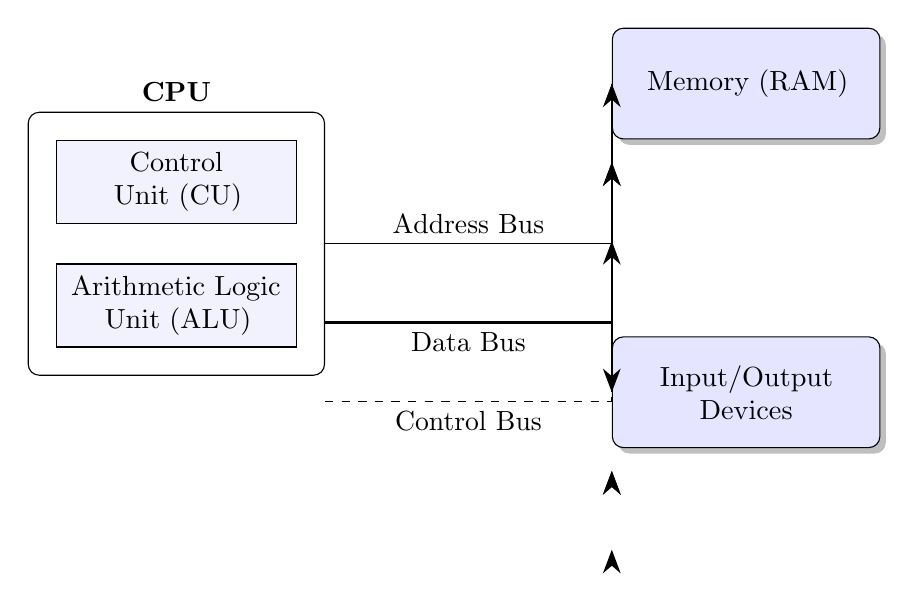
\begin{tikzpicture}[
            node distance=2.5cm,
            auto,
            main_block/.style={rectangle, draw, fill=blue!10, text width=9em, text centered, rounded corners, minimum height=4em, drop shadow},
            cpu_block/.style={rectangle, draw, fill=blue!5, text width=8em, text centered, minimum height=3em},
            arrow/.style={draw, -{Stealth[length=3mm]}},
            bus/.style={draw, <->, {Stealth[length=3mm]}-{Stealth[length=3mm]}, thick}
        ]
            % --- Place the main nodes ---
            \node[main_block] (memory) {Memory (RAM)};
            \node[main_block, below=of memory] (io) {Input/Output Devices};
            
            % --- Create the CPU block ---
            % Place the internal components
            \node[cpu_block, left=4cm of memory, yshift=-1.25cm] (cu) {Control Unit (CU)};
            \node[cpu_block, below=0.5cm of cu] (alu) {Arithmetic Logic Unit (ALU)};
            
            % Draw a box around the CPU components and label it "CPU"
            \node[rectangle, draw, rounded corners, fit=(cu) (alu), inner sep=10pt, label={[font=\bfseries]above:CPU}] (cpu_box) {};

            % --- Connect the buses ---
            % Address Bus (CPU -> Memory/IO)
            \draw[arrow] (cpu_box.east) -| node[near start, above] {Address Bus} (memory.west);
            \draw[arrow] (cpu_box.east) -| (io.west);

            % Data Bus (CPU <-> Memory/IO)
            \draw[bus] (cpu_box.east) ++(0, -1cm) -| node[near start, below] {Data Bus} (memory.west) ++(0, -1cm);
            \draw[bus] (cpu_box.east) ++(0, -1cm) -| (io.west) ++(0, -1cm);
            
            % Control Bus (CPU -> Memory/IO)
            \draw[arrow, dashed] (cpu_box.east) ++(0, -2cm) -| node[near start, below] {Control Bus} (memory.west) ++(0, -2cm);
            \draw[arrow, dashed] (cpu_box.east) ++(0, -2cm) -| (io.west) ++(0, -2cm);

        \end{tikzpicture}
        \caption{Internal Data Flow (Von Neumann Architecture)}
        \label{fig:von_neumann}
    \end{figure}
    % --- DIAGRAM PLACEHOLDER ---
    % 1. Create a diagram showing:
    %    - A box for CPU (containing CU and ALU)
    %    - A box for Memory
    %    - A box for I/O Devices
    %    - Arrows for Address Bus, Data Bus, and Control Bus connecting them.
    % 2. Save it as "von_neumann.png" and uncomment the block below.
    %
    % \begin{figure}[h!]
    %     \centering
    %     \includegraphics[width=0.7\textwidth]{von_neumann.png}
    %     \caption{Internal Data Flow (Von Neumann Architecture)}
    %     \label{fig:von_neumann}
    % \end{figure}
    
    Using the example `Total = Marks1 + Marks2`, the cycle is as follows:
    
    \begin{enumerate}
        \item \textbf{Fetch:} The Control Unit (CU) requests the first instruction (e.g., `LOAD Marks1`) from its address in RAM. The instruction travels along the Data Bus to the CPU.
        
        \item \textbf{Decode:} The CU decodes the `LOAD` instruction, understanding it needs to fetch data from the address of `Marks1`.
        
        \item \textbf{Execute (Fetch Data):} The CU sends the `Marks1` address on the Address Bus. The data (e.g., `80`) travels back from RAM on the Data Bus to a CPU register (the Accumulator).
        
        \item \textbf{Fetch/Decode:} The CU fetches and decodes the next instruction, `ADD Marks2`.
        
        \item \textbf{Execute (Add):} The CU fetches the data for `Marks2` (e.g., `90`). The Arithmetic Logic Unit (ALU) adds this `90` to the `80` in the Accumulator, resulting in `170`.
        
        \item \textbf{Fetch/Decode/Execute (Store):} The final instruction, `STORE Total`, is fetched and decoded. The CU executes it by sending the address for `Total` and the value `170` (from the Accumulator) back to RAM.
    \end{enumerate}

    \item \textbf{Evaluate the impact of memory hierarchy (cache, RAM, secondary storage) on the performance of commonly
    used applications such as video editing or gaming.} \\
    \llap{\textbf{Answer:}}
    The memory hierarchy is essential for performance, acting as a bridge between the fast CPU and slow storage. In demanding applications like gaming or video editing, each level has a distinct impact. \textbf{Cache (L1/L2/L3)} is the fastest memory, and its impact is on real-time responsiveness. In gaming, it stores frequently used instructions (like game physics), preventing "stutter" and enabling a smooth frame rate. \textbf{RAM (Main Memory)} is the medium-speed "working area." Its impact is on multitasking and handling large active files. In video editing, the OS, the software, and the active video clips must fit in RAM. If RAM is insufficient (e.g., 8GB for a 4K project), the system must constantly swap data with the disk, causing severe slowdowns. Finally, \textbf{Secondary Storage (SSD/HDD)} is the slowest level, and its impact is on loading times. In gaming, an SSD will dramatically reduce initial game load screens by transferring large assets (textures, maps) to RAM much faster than an old HDD.

    \item \textbf{Imagine you are designing a kiosk for railway ticket booking. Justify your selection of input and output
    devices based on user interaction, reliability, and efficiency.} \\
    \llap{\textbf{Answer:}}
    For a public railway kiosk, \textbf{input devices} must be robust and intuitive. The primary interface would be a \textbf{resistive touch screen}; it is chosen for high \textbf{reliability} against public use and vandalism, as it responds to pressure (unlike a capacitive screen) and works with any object. For payment, a \textbf{stainless steel PIN pad} is justified for its high \textbf{reliability} and security in entering sensitive PINs. Lastly, a \textbf{QR/Barcode Scanner} would be included for \textbf{efficiency}, allowing users to scan IDs, mobile payment codes, or existing tickets far more quickly and accurately than manual typing.
    
    The \textbf{output devices} must provide clear, fast feedback. The main \textbf{display}, integrated with the touch screen, is the primary output, providing immediate visual feedback for good \textbf{user interaction}. A \textbf{thermal printer} is the ideal choice for printing tickets. Its justification is based on \textbf{efficiency} (it's extremely fast and requires no ink/toner) and \textbf{reliability} (few moving parts), making it perfect for a high-volume kiosk. Finally, a \textbf{speaker} would be included to provide audio prompts, improving overall \textbf{user interaction} and accessibility.

    \item \textbf{You have Rs. 35,000 to assemble a personal computer for online learning and basic office work. List the
    hardware components you would choose and justify your selection based on performance and cost.} \\
    \llap{\textbf{Answer:}}
    This budget is for the PC tower only, aiming for a responsive experience for multitasking (video calls, browser tabs, Office apps). The item format is best for this answer.
    
    \begin{enumerate}
        \item \textbf{CPU: AMD Ryzen 5 5600G} (approx. Rs. 11,000)
            \textit{Justification:} This CPU is the core of the build. Its integrated Vega 7 graphics are powerful enough for smooth 1080p video calls and office tasks, completely saving the \textbf{cost} of a separate graphics card. Its 6 cores provide excellent \textbf{performance} for multitasking.
            
        \item \textbf{Motherboard: B450M or A520M} (approx. Rs. 5,500)
            \textit{Justification:} A \textbf{cost}-effective motherboard that is fully compatible with the 5600G. It provides all necessary features, including slots for NVMe SSD and 2-4 RAM sticks.
            
        \item \textbf{RAM: 16GB (2x8GB) DDR4 3200MHz} (approx. Rs. 4,500)
            \textit{Justification:} 16GB is the sweet spot for multitasking \textbf{performance}. 8GB would be a bottleneck. Using two sticks (2x8GB) enables "dual-channel" mode, which significantly boosts the \textbf{performance} of the 5600G's integrated graphics.
            
        \item \textbf{Storage: 1TB NVMe Gen3 SSD} (approx. Rs. 6,500)
            \textit{Justification:} This is the single biggest factor for "fast-feeling" \textbf{performance}. An NVMe SSD makes boot times, opening applications (Word, Chrome), and finding files near-instantaneous. 1TB offers ample space at a great \textbf{cost}-per-GB.
            
        \item \textbf{Power Supply (PSU): 450W 80+ Bronze} (approx. Rs. 3,500)
            \textit{Justification:} A reliable PSU from a brand like Cooler Master or Deepcool is critical for system stability. 450W is more than enough power for this efficient build, and the 80+ Bronze rating ensures good \textbf{cost}-efficiency.
            
        \item \textbf{Case: Basic ATX/mATX Mid-Tower} (approx. Rs. 4,000)
            \textit{Justification:} A \textbf{cost}-effective case with decent airflow to house the components.
    \end{enumerate}
    \textbf{Total: approx. Rs. 35,000}. This build prioritizes a fast SSD and 16GB of RAM, which will provide the best day-to-day performance for learning and office work.
\end{enumerate}

\textbf{Q2:}
\begin{enumerate}
  \item \textbf{Compare proprietary and open-source software models by analyzing two software products (e.g., Microsoft
    Office vs. LibreOffice) in terms of cost, accessibility, updates, and support.} \\
    \llap{\textbf{Answer:}}
    A comparison between the proprietary \textbf{Microsoft Office} and the open-source \textbf{LibreOffice} highlights the fundamental differences in their models. The most evident factor is \textbf{cost}: Microsoft Office requires a recurring subscription or a high one-time license fee, whereas LibreOffice is entirely free. This is linked to \textbf{accessibility}; Microsoft's source code is a protected trade secret, while LibreOffice's source code is open for anyone to view, modify, and distribute. This core difference dictates the approach to \textbf{updates and support}. Microsoft provides official, paid customer support and centrally controls all updates, pushing features as it sees fit. LibreOffice, conversely, relies on free, community-based support through public forums and wikis, with updates being developed collaboratively by a global volunteer community.

  \item \textbf{Assume your system has both Linux and Windows installed. Discuss three scenarios where Linux offers
    more control or flexibility compared to Windows, and explain why.} \\
    \llap{\textbf{Answer:}}
    Linux provides significantly more granular control and flexibility than Windows in many scenarios. A primary example is \textbf{system updates}. Windows often forces mandatory updates and subsequent reboots at inconvenient times. In Linux, the user has 100\% control: they can decide precisely *when* to update, *what* specific packages to update (e.g., update only the browser but not the kernel), and reboots are almost never required for updates. This control extends to \textbf{software and environment management}. On Windows, installing a development environment requires running multiple, separate `.exe` installers. On Linux, a package manager (like `apt` or `dnf`) provides a central, scriptable interface to install and manage all software, giving superior control. Lastly, Linux offers greater flexibility in \textbf{system recovery}. If a Windows installation becomes corrupt, a user can boot into their dual-boot Linux partition, mount the Windows (NTFS) drive, and have full, unrestricted access to back up all their files or even edit Windows configuration files to attempt a repair.

  \item \textbf{Reflect on how compilers and interpreters differ in handling programming errors. Provide an example where
    using an interpreter would be more beneficial during development.} \\
    \llap{\textbf{Answer:}}
    Compilers and interpreters differ fundamentally in error handling. A \textbf{compiler} (like for C++) translates the \textit{entire} program into machine code before running it. During this "compile-time" phase, it scans all files and generates a complete list of every syntax or type-checking error. The program cannot run at all until every single error is fixed. In contrast, an \textbf{interpreter} (like for Python) translates and executes the program \textit{line-by-line} at "run-time." It starts immediately, and execution only stops when it encounters a line with an error, reporting just that single error. This line-by-line approach is highly beneficial for rapid development. For example, if you are writing a data analysis script, you can run it, wait 30 seconds for it to load a large file, and then have it fail on a minor syntax error in your charting code. With an interpreter, you can fix that single line and immediately re-run, providing a much faster feedback loop than a compiler, which would force you to re-compile the entire application for every small change.

  \item \textbf{Create a scenario (e.g., preparing an event budget) where both a word processor and spreadsheet are required.
    Describe how you would use each to accomplish the task effectively.} \\
    \llap{\textbf{Answer:}}
    A perfect scenario is preparing an official "Annual College Fest Budget Proposal" for the principal. Both tools are required for an effective workflow. I would first use the \textbf{spreadsheet (e.g., LibreOffice Calc)} to handle all financial calculations. Here, I would create a detailed table with columns for `Item`, `Quantity`, `Cost per Unit`, and `Total Cost`, using formulas to auto-calculate the total for each item and a `SUM()` function for the "Grand Total." This ensures all mathematics are 100\% accurate and easily adjustable. After finalizing the numbers, I would use the \textbf{word processor (e.g., LibreOffice Writer)} to create the formal proposal document. This file would contain the formatted cover page, the event introduction, and the text justifying the budget. Finally, I would copy the completed budget table from the spreadsheet and paste it directly into the word processor. This combines the narrative and formatting strengths of the word processor with the calculation power of the spreadsheet.

  \item \textbf{Design a simple database schema to store student attendance in a classroom. Mention tables, fields, and
    types. Also, mention one project management tool and how it can help in managing a classroom project.} \\
    \llap{\textbf{Answer:}}
    A simple, normalized database schema would require two tables to avoid redundant data.
    
    \textbf{Table 1: `Students`} (Stores one record per student)
    \begin{itemize}
        \item `student\_id` (Type: `INT`, Primary Key)
        \item `first\_name` (Type: `VARCHAR(100)`)
        \item `last\_name` (Type: `VARCHAR(100)`)
        \item `roll\_number` (Type: `VARCHAR(20)`, Unique)
    \end{itemize}
    
    \textbf{Table 2: `AttendanceLog`} (Stores one record per student, per day)
    \begin{itemize}
        \item `log\_id` (Type: `INT`, Primary Key)
        \item `student\_id\_fk` (Type: `INT`, Foreign Key references `Students.student\_id`)
        \item `attendance\_date` (Type: `DATE`)
        \item `status` (Type: `ENUM('Present', 'Absent', 'Late')`)
    \end{itemize}
    
    For a project management tool, a team could use a Kanban board like \textbf{Trello}. To manage a classroom project, the group would create a Trello board with lists such as "To-Do," "In-Progress," and "Done." Each project task (e.g., "Research Topic," "Create PowerPoint Slides," "Write Script") becomes a "Card." Team members can be assigned to cards, add checklists, and set due dates. As a member begins a task, they drag their card to "In-Progress," and then to "Done" upon completion. This provides a simple, visual way for everyone, including the teacher, to track the project's progress and see who is responsible for each part.
\end{enumerate}

\textbf{Q3:}
\begin{enumerate}
  \item \textbf{You have to set up a small office network with internet connectivity. Describe the networking devices
    (router, switch, etc.) and topology you would choose and justify your decision.} \\
    \llap{\textbf{Answer:}}
    For a small office network, the best choice is a \textbf{Star Topology}, which is reliable and easy to manage. The central device would be a \textbf{Router}. I would choose an integrated "small office/home office" (SOHO) router, which combines a router, a switch, and a wireless access point into one cost-effective device.
    
    This single router serves three functions:
    1.  \textbf{Router:} It connects our entire office (the LAN) to the internet (the WAN) via the ISP's modem. It manages all traffic and acts as the DHCP server, automatically assigning local IP addresses to all devices.
    2.  \textbf{Switch:} Its built-in Ethernet ports (typically 4-8) will form the core of the star topology. All wired devices, such as desktop PCs and network printers, will connect via cable directly to these ports. If more ports are needed, a secondary, standalone \textbf{Switch} can be plugged into one of these ports to expand the network.
    3.  \textbf{Wireless Access Point (WAP):} The built-in Wi-Fi provides internet connectivity for mobile devices like laptops, tablets, and phones.
    
    This star topology is justified because it is robust; if one device's cable fails, only that device loses connection, and the rest of the network remains operational. It's also efficient and easy to troubleshoot.

  \item \textbf{Suppose you are tasked with designing a personal learning portal. Identify three internet services you would
    integrate (e.g., cloud storage, video conferencing, email notifications) and justify their use.} \\
    \llap{\textbf{Answer:}}
    A personal learning portal should centralize all aspects of a student's workflow. Three essential internet services to integrate would be cloud storage, an authentication service, and a real-time communication API.
    
    First, I would integrate a \textbf{Cloud Storage} service like Google Drive or Dropbox. This is justified because it allows the student to store and access all their course materials—notes, e-books, and assignment drafts—from any device. It also provides version history and a reliable backup, preventing catastrophic data loss from a local hard drive failure.
    
    Second, I would use a social \textbf{Authentication Service} like "Sign in with Google" or "Sign in with GitHub" (OAuth). This is justified because it enhances both security and convenience. The user doesn't need to create and remember yet another password, and the portal doesn't need to securely store user credentials, offloading that complex security burden to a trusted provider.
    
    Third, I would integrate a \textbf{Real-Time Communication} service (like WebRTC or a third-party API) for video conferencing. This is justified as it transforms the portal from a static file repository into an interactive learning hub. It enables live one-on-one sessions with tutors, participation in virtual study groups, and viewing live-streamed lectures, all from within the same interface.
\end{enumerate}

\end{document}

